\documentclass{llncs}
\pagestyle{headings}   % turn on page numbers
\usepackage{epsf}
\usepackage{epsfig}

\usepackage{url}

\newcommand{\Circus}{{\sf\slshape Circus}}
\newcommand{\Class}[1]{\texttt{#1}}
\newcommand{\Element}[1]{\texttt{#1}}
\newcommand{\Interface}[1]{\texttt{#1}}
\newcommand{\Method}[1]{\texttt{#1}}

\begin{document}
\title{CZT Support for Z Extensions}
\author{Leo Freitas$^1$ \and Tim Miller$^2$ \and Petra Malik$^3$ \and Mark Utting$^3$}

\institute{%
   \begin{tabular}{cc}
      University of York, UK  $\quad\quad$ & University of Liverpool, UK
      \\ %
      $^1$\texttt{leo@cs.york.ac.uk} $\quad\quad$ & $^2$\texttt{tim@csc.liv.ac.uk}
   \end{tabular}
   \begin{tabular}{c}
      University of Waikato, New Zealand
      \\ %
       $^3$\texttt{\{petra, marku\}@cs.waikato.ac.nz}
   \end{tabular}
} %

\maketitle


\begin{abstract}
  The Community Z Tools (CZT) is an integrated
  framework for the Z formal specification language.  In this
  paper, we show how it is also designed to support extensions
  of Z, in a way that minimises the work required to build a
  new Z extension.  The goals of the framework are to maximise
  extensibility and reuse, and minimise code duplication and
  maintenance effort.  To achieve these goals, CZT uses a variety of
  different reuse mechanisms, including generation of Java
  code from a hierarchy of XML schemas, XML templates for shared
  code, and several design patterns for maximising reuse of Java
  algorithms.
  %
  The CZT framework is being used to implement several integrated
  formal methods, which add object-orientation, real-time features
  and process algebra extensions to Z.  The effort required to
  implement such extensions of Z has been dramatically reduced
  by using the CZT framework.

  \noindent
  \textbf{Keywords}: Standard Z, Object-Z, \Circus, TCOZ, design patterns, framework,
                     AST, parsing, typechecking, animation.
\end{abstract}

\section{Introduction} \label{sec:intro}

  The Z language~\cite{isoz} is a formal specification notation that
  can be used to precisely specify the behaviour of systems, and
  analyse it via proof, animation, test generation, and so on.  
  Z was approved as an ISO standard in 2002, but currently there are few
  tools that conform to the standard.\footnote{CADiZ 
  (\url{http://www-users.cs.york.ac.uk/~ian/cadiz} is the only Z tool
  that conforms closely to the Z standard.  It is freely available, 
  but is not open source and does not aim at supporting Z extensions.}
  Z Tools (CZT) project~\cite{czt} is an open-source Java framework
  for building formal methods tools for standard Z and Z extensions.

  CZT provides the basic tools expected in a Z environment, such as
  conversion between \LaTeX, Unicode and XML formats for Z, and
  parsing, unparsing, typechecking and animation tools.
  There are also several more experimental tools under development,
  such as a Z-to-B translator and a semi-automated GUI-builder for
  Z specifications.  However, the main design goal of CZT is to
  provide a framework which makes it easy to develop new Z tools.
  This paper describes how the framework also makes it easy to develop
  tools for extensions of Z.

  In recent years, there has been an increasing interest in combining
  different programming paradigms within an uniform formal notation,
  where Z plays a central role. This has given rise to many Z
  extensions, which add features such as
  %
  process algebras~\cite{fischer-1998,fischer-2000,circus.sem:intro}, 
  object orientation~\cite{oz,ohcircus},
  time~\cite{tcoz,circus.sem:real.time2},
  mobility~\cite{circus.sem:mobility}, and so forth.

  Among these extensions, CZT supports Object-Z~\cite{oz}, a
  specification language that extends Z with modularity and reuse
  constructs that resemble the object-oriented programming
  paradigm. Such constructs include classes, inheritance, and
  polymorphism. CZT supports Object-Z in the form of parsing,
  typechecking, and other facilities.  Currently, we are working on
  extensions for Timed Communicating Object-Z (TCOZ)~\cite{tcoz},
  which is a blend of Object-Z and Timed-CSP~\cite{timed-csp}, as well
  as extensions for \Circus~\cite{circus.sem:intro}, a unified
  refinement language that combines Z, CSP~\cite{csp.books:roscoe},
  and the refinement calculus~\cite{fm.ref:morgan}, with Hoare and
  He's \textit{Unifying Theories of Programming} (UTP) as the semantic
  background~\cite{hoare.utp}.

  This paper describes the engineering techniques used in the CZT framework
  to maximise extensibility and reuse.
  Most of these techniques could also be applied to frameworks
  for other integrated formal methods, especially when the
  framework must support several different extensions of a common
  base language (like the role of Z in CZT).

  In Section~\ref{xml-schemas}, we present a method for specifying an
  XML interchange format that maximises commonality, while
  Section~\ref{java-ast-classes} presents the generation of
  \emph{Annotated Syntax Tree} (AST) classes from this XML
  documentation. Section~\ref{parsers} presents a method for
  generating parsers, scanners, and other related tools for the
  different Z extensions, and Section~\ref{typecheckers} presents
  the design of the CZT typecheckers, which are tailored for
  extendability and reuse. Section~\ref{animation} presents the
  animation method used in the CZT animator, ZLive, and discusses the
  possibility of using this to animate extensions to
  Z. Section~\ref{section-manager} presents the design of the {\em
  section manager}, an integral component of CZT that caches
  information about specifications to improve the efficiency of the
  tools, while Section~\ref{other-tools} briefly discusses other CZT
  tools. Section~\ref{sec:conclusions} concludes the paper and
  discusses the future of the CZT project.


\section{XML Schemas}
\label{xml-schemas}

  The first step in designing the CZT tools and libraries was the
  development of an XML schema that describes an XML markup for Z
  specifications (ZML)~\cite{UttEA:03}.  This is an interchange format
  that can be used to exchange parsed and even typechecked Z
  specifications between sessions and tools.

  The idea of using Z with XML has also been explored in the
  Z/Eves theorem prover~\cite{tp.tools:zeves.ref}. It allowed one to
  create a customised theorem prover with additional tactics tailored
  for a particular specification by modifying the XML representation
  of the Z specification in Z/Eves~\cite{tp.tools:zeves.api}.
  The main problem however, was the lack of a common standard.
  The effort indeed pointed to an appropriate direction tough.

  Standard Z allows specifications to be exchanged using Unicode,
  \LaTeX\ or e-mail markup.  However, implementing a parser for such
  specifications is a non-trivial task that might take several weeks
  or even months to be finished.  ZML, in contrast, can be parsed
  immediately using one of the available XML parsers like
  Xerces\footnote{See~\url{http://xml.apache.org/xerces-j/}} or
  Crimson\footnote{See~\url{http://xml.apache.org/crimson/}}.

  Tools also benefit from being able to annotate terms with type
  information, anticipated usage, comments, location, and so on.
  The ZML format allows such annotations. [TODO: are there other advantages of ZML?]

  The XML schema for ZML has been carefully designed to be extensible
  in order to allow Z extensions to profit from those advantages as well.
  The following strategies have been used to achieve this.

  The \textit{``any''} element can be used in an XML schema to enable
  instance XML documents to contain additional elements not specified
  by the schema.  This concept has been used to define annotations.
  That is, an annotation to a term can either be one of the
  annotations defined in the XML schema for Z, or any other kind of
  data.  This allows a tool builder to decide what data makes sense
  for a particular tool.

  Secondly, inheritance is used extensively throughout the XML schema.
  Abstract elements are used to provide placeholders for their derived
  elements.  For example, the abstract element \Element{Para} is the
  parent of all concrete Z paragraphs like, for example, axiomatic
  paragraphs (element \Element{AxPara}), and free types paragraph
  (element \Element{FreePara}).  This makes it easy to include a
  reference to any kind of paragraph into other elements as, for
  example, in the definition of a Z section (element \Element{ZSect})
  which contains a sequence of paragraphs.

  More important is, however, that the inheritance hierarchy defined
  in the XML schema for ZML can be extended without even touching the
  ZML schema file.  For example, the XML schema for Object-Z imports
  the ZML schema file, and defines a new paragraph for classes (element
  \Element{ClassPara}) that is derived from element \Element{Para}
  defined in the ZML schema.  Instance documents of the Object-Z
  schema can now contain class paragraphs in addition to the standard Z
  paragraphs wherever an element \Element{Para} is expected.  The same strategy has
  been used to define expression (abstract element \Element{Expr}),
  predicates (abstract element \Element{Pred}), declaration (abstract
  element \Element{Decl}) and others, making it possible for
  extensions to add new kinds of expressions, predicates, \textit{etc}.

  This can be carried on to extending an extension.  For example, the
  additional elements provided by the Object-Z XML schema are further
  extended by the TCOZ XML schema.  Again, the definitions of the elements
  for TCOZ are encapsulated into a TCOZ XML schema file, and the ZML and
  Object-Z XML schemas do not need to be modified.
  Similarly, the \Circus\ extension for CZT is encapsulated into a
  \Circus\ XML schema file that extends the main standard Z schema.
  This approach of extension via inclusion is explored throughout the
  different layers of CZT tools.
  The resulting net effect is that once one package is finished, it
  can be directly extended through inheritance, hence simplifying the
  task of extending standard Z in a great extent.

  [TODO: are there other things that make the schema extensible?]

  The use of XML in the CZT has shown as an efficient and extensible
  solution for representing a Z specification and its extensions.  The
  XML approach helps to clarify design decisions in a straightforward
  fashion.  This representation is the key for the integrated
  development and exchange of information among different Z tools.

\section{Java AST Classes}\label{java-ast-classes}

  The Java \emph{Annotated Syntax Tree} (AST) of CZT provides a tree view of
  a parsed specification using Java interfaces and classes.  This
  allows easy access to syntactical objects like, for instance,
  paragraphs, declarations, predicates, and expressions, from within
  Java programs.

  The CZT Java AST interfaces and classes were automatically generated
  from the XML schemas described in the previous section using our
  code generator \emph{GnAST} (GeNerator for AST).  The generated code
  looks similar to the code Java data binding tools like
  JAXB\footnote{See~\url{http://java.sun.com/xml/jaxb/}} or
  Castor\footnote{See~\url{http://www.castor.org/}} are producing.  The
  generated Java interfaces and classes represent the structures
  defined in the XML schema instance document.  While the main purpose
  of a Java binding tool is to provide the ability to convert from XML
  format to Java objects and vice versa, the main purpose of GnAST is
  to generate well-designed AST classes.  For example, the AST classes
  generated by GnAST support an extensible variant of the visitor
  design pattern.

  The automatic AST generation from the XML schemas alone is already a
  considerable improvement in productivity and maintainability.  For
  instance, the complete AST folder representing standard Z contains
  around $420$ Java files.  GnAST has also been used to generate AST
  interfaces and classes for Object-Z, TCOZ, and \Circus.  In total,
  from the four XML schema files for standard Z and its extensions, GnAST
  automatically generates around $2300$ Java files.  This provides a
  very convenient way to obtain AST interfaces and classes for Z
  extensions that fit well into the AST for standard Z.  That is, the
  AST classes for Z extensions also support the visitor design pattern
  described below.

  The visitor design pattern~\cite{GamEA:95,MaiCha:01} makes it very
  easy to write tools like typecheckers and printers, that need to
  traverse an AST.  It provides a way to separate the structure of a
  set of objects from the operations performed on these objects.  This
  allows a new operation to be defined without modifying the AST
  classes.  To define a new operation, all you need to do is to
  implement a new visitor class.

  The visitor design pattern used in CZT has been described in detail
  in~\cite{czt}.  It is a variant of of the \emph{acyclic
  visitor}~\cite{Mar:97} pattern and the \emph{default
  visitor}~\cite{Nor:97} pattern.  Its main advantages are that it
  allows the AST interfaces and classes to be extended without
  affecting existing visitors, and that it allows a visitor to take
  advantage of the AST inheritance relationships.

  This has a big impact on the applicability of visitors for
  extensions like Object-Z, TCOZ, and \Circus.  It firstly makes sure
  that the Z AST classes can be extended without having to modify
  existing Z visitors like typechecker, printer, \textit{etc}.  It is a
  prerequisite for CZT to be extensible.  The second feature makes it
  easy to reuse existing visitors in extensions.  By defining default
  behaviours for abstract classes, it is possible to implement tools
  that are applicable to all extensions.  For example, a copy visitor
  that copies an AST can provide a default behaviour for
  \Interface{Term}, the base of the AST inheritance hierarchy.  Since
  AST classes for extensions also derive from \Interface{Term}, this
  copy visitor works for any extension.  If the default behaviour of a
  visitor does not provide the required functionality for a particular
  class, it can be simply overwritten by providing a new method with
  the required functionality for this class.

  [TODO: examples of visitors?]

  This flexibility and independency of the CZT visitor has also been
  shown to be very useful during the development of new tools.  By
  providing default behaviour, it is possible to concentrate on
  specific aspects of the language and ignore others.  This allows for
  rapid prototyping and eases debugging.

\section{Parsers, Scanners, and Related Tools}
\label{parsers}

  CZT includes a suite of important tools for operations such as
  parsing, typechecking, and markup conversion. In addition to a
  parser and typechecker for Z, an Object-Z parser is provided, and
  \Circus\ and TCOZ parsers, as well as Object-Z and \Circus\
  typecheckers, are under development.  The Object-Z, TCOZ, and
  \Circus\ tools extend the Z tools by adding support for the
  additional constructs these languages provide.  As each language is an
  extension of Z, it is tempting to just keep adding to the tools
  for each extension, and use the largest superset of all
  extensions. For example, use the TCOZ tools to parse and typecheck
  Z. However, this has two distinct problems. Firstly, one aim of the
  CZT project is to create tools that strongly conform to the Z
  standard, so allowing extra constructs to be parsed and different
  type-rules will break the strong conformance. Secondly, the
  extensions of Z are not linear. For example, Object-Z extends Z with
  class paragraphs, and TCOZ extends Object-Z with concurrency
  operators, but \Circus\ extends neither of these --- only
  Z. Therefore, CZT requires an approach that produces separate tools
  for each Z extension, maximises the commonality between the parsers,
  and minimises versioning and maintenance problems via reuse.

\subsection{Parsers and Scanners}

  CZT includes parsers for standard Z specifications given either in
  Unicode or using \LaTeX\ markup.  Support for e-mail markup is
  planned. To produce different parsers and scanners for Z and its
  extensions, CZT uses XML templates, and generates the code from these
  templates using XSLT, a language for transforming XML\footnote{See~\url{http://www.w3.org/TR/xslt}}. Java
  Cup\footnote{See~\url{http://www.cs.princeton.edu/\~{}appel/modern/java/CUP/}} is
  used to generate the CZT parsers from an LALR grammar, and
  JFlex\footnote{See~\url{http://jflex.de/}} is used to generate the
  scanners.

  Unfortunately, it is quite difficult to reuse code from an
  automatically generated scanner or parser, and neither Java Cup nor
  JFlex explicitly supports inheritance for parser or scanners
  respectively.  To avoid duplicated code, XML templates that contain
  the different parser and scanner variants are used. From this, the
  different Java source files for each Z extension are generated using
  XML translation tools.  This maximises the commonality between the
  parsers and minimises versioning and maintenance problems.

All parser and scanner variants are maintained in two master XML
files: one for the parser and one for the scanner. Each master file
contains several XML tags that are used for substituting text for each
Z extension. For example, the {\tt <package/>} tag is placed wherever
one would normally write the Java package name, so that each parser
and scanner can be contained in their own package. The tags {\tt
<add:}{\em extension}{\tt >} and {\tt </add:}{\em extension}{\tt >}
are used to wrap around code that are specific to particular Z
extensions. Thus, to add a new type of expression to the Object-Z parser,
one would add a new production to the appropriate grammar rule in the
master file, and place it between the {\tt <add:oz>} and {\tt
</add:oz>} tags.

To generate the individual Java Cup files for each extension of Z,
XSLT is used to include the necessary code, and to substitute in
values for tags. For example, to generate the Object-Z parser, XSLT is
applied to the master file, and supplied with the three arguments
below:
\begin{enumerate}
  \item {\tt "class"} substituted with {\tt "Parser"}.
  \item {\tt "package"} substituted with {\tt "net.sourceforge.czt.parser.oz"}.
  \item code in {\tt "oz"} tags to be included.
\end{enumerate}

Similar rules are specified for each parser and scanner variant. The
result is a series of Java Cup and JFlex files, one for each language,
which can then be used to generate the parser and scanner code.

The use of XML templates enables parsing code to be reused and easily
maintained.  Extending the parser and scanner for a new language can
be done by just adding the respective grammar and lexer rules together
with few modifications such as those parameters above.  For example,
we are experimenting the incorporation of the available \Circus\
parser~\cite{circus.other:parser} rules within the flexible CZT
framework. The obvious advantages are the widely tested and supported
standard Z classes, \LaTeX\ markup and Unicode, visiting and other
facilities.

\subsection{Multiple Markups}\label{multiple-markups}

 CZT supports multiple markups for each Z extension.  The different
 markup languages suit different communities.  For example, \LaTeX\ is
 preferred by researchers while Unicode WYSIWYG editing might be more
 attractive for students or industrial users. At present, Unicode,
 \LaTeX, and the XML format are supported.  Adding additional markups
 is straightforward, as this section will present.  XML markup is not
 considered any further because it can be parsed immediatly using
 existing XML parsers.  CZT uses
 JAXB\footnote{See~\url{http://java.sun.com/xml/jaxb/}} to unmarshal an
 XML document into a tree of Java objects, and then uses the visitor
 design pattern to convert this tree into an AST.

In order to avoid having to provide a parser for each markup language,
all specifications are first translated into Unicode and subsequently
parsed by a Unicode parser\footnote{See \cite{czt} for a more detailed
description of the parser architecture.}.  This also makes sure that
names in the AST are markup independent: they are represented in
Unicode independently on the actual markup used in the source
document.  This is a necessary precondition to allowing different
sections of a specification to be written in different markups.

A consequence of this architecture is that extensions of Z need
to support at least Unicode.  CZT provides a Z Unicode scanner, which
performs lexical analysis on a Unicode stream and breaks it into the
necessary tokens.  A scanner for a Z extension can be derived by
adding additional scanner rules to the CZT scanner template as
described above.  In order to support \LaTeX\ markup, it is convenient
to provide a \LaTeX\ toolkit section for a given extension.  In
addition to defining new operators, these \LaTeX\ markup documents
contain \LaTeX\ markup directives~\cite{isoz,czt} used to specify how
certain \LaTeX\ commands are to be converted into Unicode.  The
\LaTeX\ to Unicode translator parses these definitions and converts
each \LaTeX\ command into the corresponding Unicode sequence.
However, \LaTeX\ \verb+\begin{xxx}+ and \verb+\end{xxx}+ commands
cannot be defined using \LaTeX\ markup directives.  If a Z extension
needs to provide new paragraphs, the \LaTeX\ to Unicode converter
needs to be adapted directly.  Again, this is possible by adding new
rules to the converter template file.


%The CZT parsers are markup independent, but all of our scanners
%provide their respective parsers with Unicode when scanning Z variable
%names, for instance. The reason for this is straightforward: Z specifications
%are made up of sections, with each section having a name and a list of
%parent sections. The definitions in a parent section are included in
%the child section for a specification. For example, the Z toolkit is
%specified as a series of \LaTeX\ sections. Now, consider the case in
%which a person would like to use the Z toolkit, but would like to use
%Unicode for their own specifications. This would require CZT to
%provide a Z toolkit in Unicode, because the names used for
%declarations in the Z toolkit would be in \LaTeX~instead of
%Unicode. To work around this problem, all markups are converted to
%Unicode, therefore allowing different sections of a specification to
%be written in different markups.

%With this architecture, each Z extension can also provide its own
%particular toolkit extension given as a \LaTeX\ specification file.
%The extended toolkits usually contains keywords, special symbols, and
%commonly used functionality described with standard Z templates, for
%instance.

%Therefore, CZT provides a Unicode scanner, which performs lexical
%analysis on a Unicode stream and breaks it into the necessary
%tokens. CZT's \LaTeX~scanner, instead of implementing all of the
%scanner rules, converts its \LaTeX~stream into a Unicode stream. In
%addition to solving the problem discussed above, this greatly
%simplifies the \LaTeX~scanner, because much of the conversion is
%straightforward in comparison to scanning Z tokens. Moreover, location
%information is recorded in the ASTs using annotations on each of the
%nodes, and this points to the location in the original specification file.

%Of course, the \LaTeX~to Unicode scanner needs to know how to convert
%\LaTeX~tokens into Unicode. This is done by specifying, in the \LaTeX\
%file that the token is first used, the corresponding Unicode
%representation for each \LaTeX~token used. For example, in the Z
%toolkit \LaTeX~file, the following rule is written specifying the
%\LaTeX\ token for powerset (\verb+\power+):
%\begin{verbatim}
  %%Zprechar \power U+2119
%\end{verbatim}
%
%The {\tt \%\%Zprechar} keyword specifies that \verb+\power+ is a
%prefix character that always has a hard space after it, and that its
%Unicode equivalent is U+2119. There are
%similar operators for postfix, infix, and nofix characters, as well as
%words.

%An additional component parses these definitions, and records this in
%a symbol table. Each time a \LaTeX~token is read, a lookup is
%performed on this table to find the Unicode mapping. If the lookup
%fails because the token is not in the table, a warning is issued, and
%the \LaTeX~token is used, minus the \verb+\+ token at the
%front. Therefore, for each new \LaTeX~token introduced into a
%specification, a unique Unicode mapping must be provided for the
%\LaTeX~to Unicode scanner, or be content with using the \LaTeX~token's
%base name.

%The price to pay for such flexibility is a slower parsing experience.
%We are currently working on ways around this performance penalty.  One
%possible optimisation is to have the option to use hard-coded versions
%of standard sections such as the Z toolkit.
%That means, a large singleton~\cite{GamEA:95} class that mocks up
%the parser (or even the typechecker) job.
%The benefit is simple:~the ``parsing'' time can be reduced to a minimum
%of class loading and object instantiation.
%Moreover, inheritance can be used for the extensions' toolkits, as well as
%the visitor pattern to automatically generate the hard-coded files similarly
%to the way GnAST works. Since most Z section
%specifications do include the Z toolkit, then this should improve
%parsing performance considerably because no parsing will be necessary
%for the Z toolkit included as a parent of other used-defined Z
%sections.  This notion can be generalised for other Z extensions,
%provided their extended toolkits reach an enabling level of stability.

Another advantage of this approach is that to parse a specification
written using a new markup, for example, the e-mail text-based markup,
one only has to implement an e-mail to Unicode scanner. In addition,
the scanners can function as converters between different markups
without have to parse the specifications. This simplifies many other
tools in the suite as well. For example, the CZT tool suite provides
printing of abstract syntax trees into the different markups. However,
instead of implementing a printer for each markup, only a Unicode
printer is implemented, and converters are used to print the other
markups.

  \begin{itemize}
    \item[Petra] Below is another version of this section.  I started
    with a few changes and ended up rewriting everything.  No idea
    what to do now ...
    \item[Tim] Very nice, Petra! I've merged this in with the first
    few paragraphs, and the last paragraphs from the ones we have
    earlier.
    \item[Leo] It is nice indeed!
    What about the last commented paragraph?
    If we agree on this performance point (and the possible solution),
    I think it is a good idea to mention it. I've included something else
    after a revision that I will include to the commented paragraph.
  \end{itemize}

\section{Typecheckers}
\label{typecheckers}

Typecheckers in CZT are written in a much different way from the parsers
and scanners. Each Z extension has its own typechecker, and while reuse
is of high importance, using XML templates is unnecessary because
differently from the parsers, Java interfaces and inheritance can be used to
extend the typecheckers.

The Z typechecker is the base implementation. Most of the typechecker
is written using visitors, which can be extended as discussed in
Section~\ref{java-ast-classes}. There are a few additional classes
that are used, such as the class that performs the unification of two
types for type inference and for checking type consistency. If the
specification is type-correct, the product of the Z typechecker is the
original AST annotated with type information as defined in the ISO
standard~\cite[Section~10]{isoz}.  If not, the result is the parsed AST
together with a list of messages outlining the type errors.

The typechecker is designed for extendability. Application of the type-rules
is implemented using visitor classes. While it is tempting to
write the typechecker as one large visitor, this creates maintenance
problems as this visitor would be quite large.  In order to enable
code reuse within the typechecker architecture, we allow each language
entity to be checked by independent checker classes.  Currently, for
the standard Z typechecker, we have an individual checker for
sections, expressions, predicates, declarations, and paragraphs. Each
of these checkers implements visitors for the corresponding AST hierarchy
subtree.  These will be referred to as the {\em type-rule visitors}.

This does not only enable reuse, but also increases modularity and
maintainability.  For example, additional functionality, such as post
checking for unresolved set and reference expressions that may
introduce an unresolved type, are implemented in the same way with
another checker. This post checker ensures that all implicit
parameters such as generic actuals have been completely determined.
Furthermore, from the development point of view, it allows (possibly
different) teams to implement different language entities, and/or
development through iterations.  This also provides a good aid for
debugging as one can guarantee the conformance of each checker, hence
isolating (if not minimising) debugging efforts.

However, the type-rule visitors require access to shared resources,
such as typing environments and the class for type unification, as
well as common ``helper'' methods used throughout the implementation
such as error reporting.  So, each type-rule visitor inherits an
abstract class called {\tt Checker} containing such shared
functionality.

Each type-rule visitor implemented through individual {\tt Checker}
subclasses are blended together in the {\tt TypeChecker} class
containing references to all required shared resources. They have an
aggregation-by-reference relationship.  That is, each type-rule
visitor is constructed and owned by the same instance of {\tt
TypeChecker} for each copy of the typechecker that is running.  Each
type-rule visitor is passed a reference to their parent {\tt
TypeChecker} so they are able to call visit methods on each other.  Of
course, this could all be implemented without the {\tt TypeChecker}
class by just passing each resource to a subclass, but the approach
that has been implemented allows extensions to the typechecker to
reuse constructors and other initialisation code, as well as different
type-rule visitors and ``helper'' methods.

For example, for type checking a schema-text of an {\tt AxPara} for,
say an axiomatic definition, the {\tt ParaChecker} class implementing
the type-rule visitor of Z paragraphs needs to type check both the
declarations and the predicate parts.  Although visiting through the
given AST is the general solution, the typechecking of the
declarations part is delegated to the {\tt DeclChecker} class, whereas
the typechecking of the predicate part is delegated to the {\tt
PredChecker} class.  The {\tt DeclChecker} in turn uses the {\tt
ExprChecker} to ensure that expressions defining the declaring
variables type are well-formed.  Moreover, as the job of each {\tt
Checker} class is distinct, it is easier to establish an uniform
visiting protocol. For instance, all the visiting methods of the {\tt
ParaChecker} class, which typechecks the AST hierarchy tree from the
{\tt Para} abstract class, returns a {\tt Signature} of name and type
pairs declared in that {\tt Para}. Similarly, the {\tt DeclChecker}
class typechecks the {\tt Decl} subtree returning the list of name and
type pairs that will form the {\tt ParaChecker} signatures.  As one
would expect, the {\tt PredChecker} class typechecks the {\tt Pred}
subtree returning the type unification result, and the {\tt
ExprChecker} class typechecks the {\tt Expr} subtree returning a {\tt
Type} with resolved reference parameters, in which type unification
has already taken place.

To extend the Z typechecker, a new package is created, say {\tt oz}
for an Object-Z typechecker.  In this package, a new {\tt oz.Checker}
class is implemented, which inherits the base {\tt z.Checker}
class. In this new class, any common methods that are to be used by
the extended typechecker are implemented, and existing methods are
overridden or overloaded if additional functionality is needed.  Then,
new type-rule visitors are created, one for each language entity that
requires an additional type-rule visitor.  These type-rule visitors
implement the visit methods only for additional constructs in the
language, or for constructs in the base language that may have
additional constraints. Clearly, this does not handle constructs in
the base language.

As far as code reuse is concerned, this is the point where our design
with distributed checkers for each language entity managed by a
centralised {\tt TypeChecker} class pays off.  For each new type-rule
visitor, say the {\tt oz.ExprChecker} class, an instance to the
corresponding visitor of the base language ({\tt z.ExprChecker}) is
created. Therefore, Object-Z expressions are handled by the {\tt
oz.ExprChecker} class, whereas Z expressions must be handled by delegation
to the {\tt z.ExprChecker} class.  To enable this idea to work, we rely on
the general visiting protocol described in Section~\ref{java-ast-classes} and in~\cite{czt}.
That is, firstly {\tt oz.ExprChecker} catches all Object-Z expressions.
Secondly, an additional visit method is implemented --- one that
``catches'' all AST nodes for the base language ---, and the base
type-rule visitor is used to typecheck these nodes.  For example, in
the {\tt oz.ExprChecker}, apart from the Object-Z expressions
visiting methods, an additional visit method for remaining {\tt Expr}
is implemented as
%
\begin{verbatim}
  private z.ExprChecker zExprChecker_;
  ...
  public Object visitExpr(Expr expr) {
    return expr.accept(zExprChecker_);
  }
\end{verbatim}
%
Therefore, when {\tt oz.ExprChecker} does not implement a visit method
for a particular expression, it calls the instance of {\tt
z.ExprChecker} to visit that expression, hence reusing the code
implementation for the base language.  Finally, a new {\tt
oz.TypeChecker} class, which inherits the base {\tt z.TypeChecker}, is
created aggregating (by reference) the new type-rule visitors.  Since
it inherits from the {\tt z.TypeChecker}, the original type-rule
visitors are accessible to enabled the extended typechecker to forward
type-rule visitors to the base typechecker.  Because visitor
interfaces are used, the underlying implementation of the extended
typechecker need not inherit from the base typechecker, and the way to
access these type-rule visitors via the {\tt TypeChecker} class
remains the same.  So, a statement in a type-rule visitor asking
an {\tt Expr} to accept a visitor would be written:
%
\begin{verbatim}
  Type2 type = (Type2) expr.accept(exprChecker());
\end{verbatim}
%
The method {\tt exprChecker()} returns a {\tt Checker} instance, and
is implemented in {\tt z.Checker}. It is shorthand for the expression
type-rule visitor inside the {\tt TypeChecker} object. Therefore, the
visitor that this {\tt Expr} accepts is based on the runtime value of
that object, which in the case of the Z typechecker, would be an
instance of {\tt z.ExprChecker}, but in the case of the Object-Z
typechecker, would be an instance of {\tt oz.ExprChecker}.


To help clarify this scenario, we present the design of the Z
typechecker, and the Object-Z typechecker that extends
it. Figure~\ref{tc-design} presents a UML-like outline of the class
design. From this figure, one can see that the class {\tt oz.Checker}
inherits from {\tt z.Checker}, and then the type-rule visitors inherit
from their respective {\tt Checker} class.
%
\def\epsfsize#1#2{0.70#1}
\begin{figure}[t]
\begin{center}
\epsfbox{tc-design.eps}
\caption{Individual checkers}\label{tc-design}
\end{center}
\end{figure}
\def\epsfsize#1#2{\epsfxsize}
%
Although this is an unusual design, it is clear that it provides good and elegant support for extension.
An alternative approach is to extend the base type-rule visitors for each new type-rule visitor.
However, this means that the common code implemented in the {\tt Checker} class must all be
implemented in the base {\tt Checker} class, which requires a strong coupling between
all of the typecheckers.

Other components of the typecheckers are also extended using
inheritance.  For example, the class for type unification is extended
by overriding the {\tt unify} method in that class.  It takes two {\tt
Type}s as parameters and attempts to unify them, returning whether the
unification was successful, partial (unification did not fail, but
there are still unresolved types), or failed.  For Object-Z, an
additional type is needed to handle instances of classes.  The
overriding method first checks if the types of class types, and
attempts unification on them.  If they are not unifiable, the
overridden method is called using the {\tt super} keyword.

In general, provided that type and scoping-rules are available, this
recipe can be used for other extensions as well.  For example, an
initial typechecker environment for \Circus\ has been developed
following the guidelines for Z and Object-Z. Although the formal
type-rules for \Circus\ are under
development~\cite{circus.other:typechecker}, we already have a
prototype version of a \Circus\ typechecker.  Provided the
architecture and the design decisions are understood, the
implementation task is relatively straightforward, and directly
benefits from code reuse and elegant object-oriented design.  In
practice, after understanding the design, creating the prototype
typechecker for \Circus\ took a couple of days, with the author of the
\Circus\ typechecker having not previously seen the Z
typechecker. The obvious advantage is that by inheriting from the
base Z typechecker, the prototype already enforces standard Z
type-checking conformance. Once the additional type-rules for \Circus\
are available, extending the prototype for a full compliance typechecker
should be straightforward.


\section{Animation}
\label{animation}

    Further to parsing and typechecking standard Z and its extensions, CZT also includes
    animation facilities. Z animation is particularly useful for testing, rapid prototyping,
    and experimenting. These facilitates the tasks of debugging and exploring early
    specifications in order to ensure that they meet the informal requirements.
    Moreover, it also provides a user-friendly way to present a formal Z specification
    to users with no prior Z knowledge such as students and industrial users.

    Apart from rapid prototyping, another main advantages for animating Z specifications
    are finite theorem proving (or theorem testing), and model checking.
    These enable one to search for a particular solution, or a counter example.
    Yet restricted to finite state models, it allows validation, verification, and
    experimentation with Z specifications.

    Another important aspect about Z animators is the conformance with the Z standard.
    That is, available animators do not handle some constructs, or even worst, deal
    wrongly with less used ones such as definite descriptions ($\mu$).
    An extensive discussion and comparison about Z animation tools available are given in~\cite{utting-jaza}.

\subsection{Animation Engine}

    As the CZT already implements parsing and typechecking for standard Z,
    a typechecked AST is already available for the CZT Z animator:~ZLive.
    ZLive is an animator capable of evaluating predicates and expressions using
    mode and subtype analysis~\cite{winikooff98}.
    Mode analysis is a procedure that determines the possible modes that a
    Z term can be evaluated. It works much like the solutions for a system of linear equations.
    Mode analysis consists of including additional (type and formulae ordering) information not
    present in specifications, which enable evaluation and animation.

    The tool expects a typechecked CZT AST corresponding to the Z specification to animate
    as input. Its architecture is based on a previous Z animator implemented in
    Haskell\footnote{See~\url{http://www.cs.waikato.ac.nz/~marku/jaza/}}.
    The ZLive architecture is divided into six tasks.
    Firstly, a target expression within the loaded specification is given.
    Secondly, the definitions are unfolded so that schema inclusions and toolkit operations
    are grounded to base terms. Next, the unfolded definitions are flattened into atomic
    predicates, hence reducing the specification to a normal form.
    After that, possible evaluation modes are calculated for each flatten predicate.
    This also includes an estimated number solutions.
    These moded-predicates are then reordered to the cheapest solution order in terms of
    number of solutions. Finally, all solutions are lazily enumerated as requested.

    ZLive currently supports the following flattened predicate constructs: arithmetic operators
    such as $-$, $+$, $*$, $\leq$, $<$, $\mathtt{div}$, $\mathtt{mod}$, and $\mathtt{succ}$;~set
    representations for comprehension, ranges, and displays;~most logic ($\forall$,
    $\exists$, $\lnot$, $\land$), and set operators ($=$, $\in$, $\#$);~unfolding of simple
    definitions; ~tuples, schema bindings and constants.
    We are working to include other set operators such as $\cup$ and $\cap$ soon.
    While performing mode analysis, the main issue is to find the best mode with respect to
    the complexity of solutions it represents. At the moment ZLive only implements three modes:~all-free
    variables-defined, where the solution is just a matter of fiddling;~functional, where all inputs are known
    and one output is calculated;~and one-input mode, where at least $n-1$ variables must be defined
    regardless the orders. At the moment no predicate reordering is being performed.
    We expect to include predicate reorder using $A^*$ or topological-sort algorithms,
    as suggested in~\cite{winikooff98}.

    We are currently experimenting with ZLive within the development of a model checker
    for \Circus~\cite{circus.mc:leo}.
    Thus, we plan to extend the available flattened predicates in order to cover most
    frequently Z constructs used in \Circus\ specifications.
    We also expect to include in ZLive predicate transformers, schema unfolding, and a
    tactic language in the spirit of ANGEL~\cite{z.others:angel}.
    These last improvements can form the basis of an open-source cross-platform
    theorem prover (or tester) in Java for Z (and possibly its extensions) in Java within
    the CZT framework.

\subsection{Building GUI for Z Specifications}



    CZT also contains an automatic graphical animator front-end for Z~\cite{daley2003}.
    It is a GUI builder for Z specifications that uses ZLive (or any other engine)
    for animation, and is based in \textit{Java Beans}~\cite{javabeans},
    \textit{Java Script}\footnote{See~\url{http://www.w3schools.com/js}},
    and the CZT AST classes. \textit{Java Beans} enables arbitrarily complex user interfaces,
    \textit{Java Script} enables arbitrarily complex interface behaviour, where the CZT AST
    plays a central role as the underlying format for animation and persistence through ZML.
    This allows the generation of different interface styles by varying the underlying
    Java Beans properties, where the actual behaviour keeps being managed in the same way
    by the underlying animation engine \textit{e.g.}, ZLive.

    The main goals of the tool is to provide open-source cross-platform, saveable, and
    customisable GUI front-ends with little or no programming effort, where the
    history of animation states are managed and controlled by the
    user interface animation tool.
    Once more, XML markup is used as the file format for interfaces to be saved.
    This allows, for instance, persistency implementation and animation sessions
    to be replayed.

    The tool is divided in three stages:~(i)~GUI generation, (ii)~GUI customisation,
    and~(iii)~GUI animation. The generator automatically provides a default GUI front-end
    for Z specifications. As Z can be animated in different ways, the designer allows the
    user to manually build (or customise) the generated user interface using few button clicks,
    but direct programming (or scripting) is also an option.
    Finally, the animator attaches to any underlying animation engine (in the case ZLive),
    hence enabling the actual animation.

    As occurred for other CZT tools, the front-end generator is also built for extension.
    Since it is based on the CZT AST classes and ZML markup, it already opens the possibility
    for GUI front-end animation for other CZT Z extensions such as Object-Z or \Circus.
    This is another argument that strengthens the idea of an interchangeable format with
    the CZT AST classes and ZML markup, since other Z extensions can also directly benefit
    from GUI front-end animation. Therefore, extending the tool for Object-Z
    or \Circus\ is possible. That is only possible because all tools share the same
    representation of a Z specification, namely the ZML markup (or the CZT AST classes).

\subsection{Animating \Circus}

    Another interesting task under development is the use of ZLive within the \Circus\ model checker
    in order to evaluate the Z part of \Circus\ specifications~\cite{circus.mc:leo}.
    As already mentioned, \Circus\ is a unified language~\cite{circus.sem:intro} tailored for refinement
    that combines Z, CSP~\cite{csp.books:roscoe} and the refinement calculus~\cite{fm.ref:morgan}
    using the \textit{Unified Theories of Programming}~\cite{hoare.utp} as the semantic background.
    Among other aspects, we are particularly interested in integration of model checking and
    theorem proving facilities for \Circus. In this direction, animation plays an important part
    in the evaluation of Z terms used to describe state aspects of dependable and distributed systems.

    The \Circus\ model checker architecture is divided into four main tasks as shown in Figure~\ref{mc-stages}.
    The first two involve parsing and typechecking. They use the CZT tools described in earlier
    sections. The last two stages involve the construction of a \textit{Predicate Transition System}
    (PTS) that finitely represent (possibly infinite specifications) base on the operational semantics
    of \Circus~\cite{circus.mc:opsem}, and a refinement engine that integrates refinement model checking
    algorithms together with theorem proving facilities.
    %
    \begin{figure}[t]
    \begin{center}
    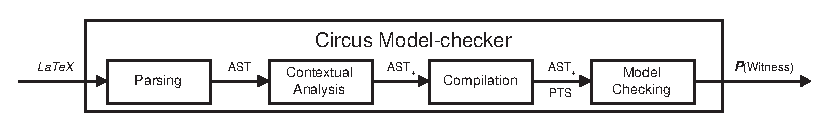
\epsfig{clip=, scale=0.9, file=mc.arch.stages.eps}
    \end{center}    \caption{\Circus\ Model Checking Stages}\label{mc-stages}
    \end{figure}
    %
    The theorem proving module presents both in the compiler and refinement engine dispatches requests
    for evaluation of Z expressions and predicates as verification conditions over the state operations
    defined in Z, or possible enabling paths available for investigation from the behavioural actions
    given using CSP.
    At this point theorem proving is usually necessary to discharge proof obligations, and simplify
    expressions or predicates. Nevertheless, for specifications with simple state operations, animation
    is also a good idea that can improve the automation of the model checking process.

    The role ZLive plays in this architecture is to tackle the requests to evaluate
    Z expressions and predicates from the compiler and refinement engine.
    As the operational semantics of \Circus\ is given in Z itself, we can use ZLive as a
    meta-level animator for simple specifications, hence enabling automatic model checking
    of state-rich \Circus\ specifications.
    With few improvements and extensions to the current implementation of ZLive to handle
    more of the schema calculus, we expect this to be a good example of how to integrate
    different CZT tools across different paradigms and tool boundaries. Furthermore,
    as the theorem proving integration architecture of the \Circus\ model checker allows pluggable
    solutions suitable for individual contexts, if ZLive cannot handle some complex \Circus\
    specifications, we can still resort to some alternative solution such as SAT solvers,
    and general-purpose theorem provers.

\section{Section Manager}
\label{section-manager}

    \begin{itemize}
        \item[Leo] A sentence about what the section manager is (abstractly) would be good.
                    I reviewed this section and pointed some unclear points, what do you think?
        \item[Petra] Good points you raised; thanks for reviewing, Leo.
        \item[Petra] I wonder whether the name ``section manager'' is
                     appropriate.  What about something like data
                     manager, specification manager, cache, session
                     manager, ...
	\item[Mark] Yes, I like SpecManager, personally (sounds a bit
		more high-level than SectionManager, and generic enough
		that it is applicable to all the Z extensions as well.
    \end{itemize}

  One of the core components of the CZT framework is the 
  \emph{section manager}, which is an extensible repository for
  formal methods objects.
  Most of the tools mentioned in the previous sections use the
  section manager to enquire about specific aspects of a
  specification.  For example, to be able to parse a Z section, the Z
  parser needs the operator definitions of the parent sections.  In
  order to typecheck a Z section, the section must be parsed and the
  parents of that section typechecked.  To print a Z section in
  \LaTeX\ markup, the operator definitions and \LaTeX\ markup
  directives of the parent sections are needed.

  While it would be possible to hard-code these dependencies and let, for
  example, the \LaTeX\ markup printer call the parser for the parent
  sections directly, it is more convenient, extensible, and efficient
  to have a central repository that is responsible for this task.
  The CZT section manager caches information about all the
  specifications and Z sections that are being processed and
  automatically runs tools such as markup converters, parsers and
  typecheckers when necessary.  The caching of the parsed form of
  commonly used objects, such as standard toolkit sections, avoids
  repeated parsing and analysis of these objects and can give significant
  performance improvements.  Abstractly, the cache is a
  mapping from a key to the actual data.  The key is a $(String,Class)$ pair,
  where the $String$ is usually the name of the section, and the $Class$ is
  the Java class of the type of data associated with this key.  This allows
  several different kinds of objects to be associated with one section,
  and provides some dynamic type security.
  For example, the Z parser adds the AST of a specification 
  it has parsed to the section manager.  The type of a Z section in Java is
  \Interface{ZSect.class}. Thus the AST for a section called \texttt{foo} is
  cached under the key \texttt{(``foo'',~ZSect.class)}.

  The CZT section manager supports two important kinds of extensibility:
  \begin{description}
  \item[Type Extensibility:] Z extensions can easily use the section
    manager to store new types of information, since the flexible
    $(String,Class)$ key system allows arbitrary Java objects to be stored
    and retrieved.  That is, the kinds of objects managed by the section 
    manager is open-ended, rather than being a fixed set of Z-related objects.
  \item[Command Extensibility:] A Z extension can easily add or override
    the \emph{default commands} of the section manager.  
    The default commands of the section manager are responsible for
    automatically computing requested objects;~they are
    implemented using the command design pattern~\cite{GamEA:95}. For
    example, if the AST (i.e. data of type \Interface{ZSect.class})
    for section \texttt{foo} is required and has not already been
    cached, the Z parser is called by the section manager in order to
    parse the specification file containing section \texttt{foo}.
    Here, the Z parser is the default command to compute data of type
    \Interface{ZSect.class}.  A Z extension that needs to use a different
    parser can simply override the default command associated with
    the type \Interface{ZSect.class}.  For example, the section
    manager can be configured to always use the Object-Z parser.
    \end{description}

  A major advantage of this default command approach is that it simplifies
  tool development and makes tools more flexible, because a particular
  tool does not have to know which other tools to use in order to
  find information about a section --- it simply requests the key that
  it wants and the section manager will locate the information if it is able.
  This gives a more flexible, \emph{plugin} style of tool development.


\section{Other Tools}
\label{other-tools}

\begin{itemize}
    \item[Leo] Shall we mention the zpatt package here as well?
\end{itemize}

\subsection{From \Circus\ to Java}

\begin{itemize}
    \item[Leo] Should it be here or in the future work section?
\end{itemize}

There is ongoing research in a translation strategy from \Circus\ to Java~\cite{angela-2005}.
In a \Circus\ specification, CSP operators given as actions, as well as Z paragraphs are intermixed.
The strategy expects a concrete \Circus\ specification refined using both CSP and Z refinement laws
using tools such as FDR~\cite{csp.tools:fdrm} and a Z refinement tool~\cite{angela-2003}.
The approach for translation is basically to traverse an AST representing the \Circus\ specification,
recursively applying the refinement steps to the concrete specification in
order to get closer to what the Java code would look like~\cite{marcel-2004}.

The requirements of the translation tool are well-defined by the translation strategy.
The implementation and verification is based on a series of case studies written using \LaTeX\ markup.
The tool will be used to perform the verification of the some of the translation laws given in~\cite{marcel-2004}.
The verification technique employed is similar to the one given in~\cite{welch-martin2000}.
However, instead of CSP it uses \Circus, and instead of model checking with FDR~\cite{csp.tools:fdrm} it
uses the refinement calculus~\cite{fm.ref:morgan}.
This will form the bases for a \Circus\ model for Java.

With the construction of further tools for \Circus\ such as a model checker~\cite{circus.mc:leo},
and a theorem prover~\cite{circus.sem:pp}, these refinement stages can be done in a much more
integrated fashion with less expressibility and semantic compromises due to restrictions among
different tool input formats and semantics.
In this scenario, the CZT tools could play an important integrating role.

For the CSP parts, the translation strategy uses JCSP~\footnote{See~\url{http://www.cs.ukc.ac.uk/projects/ofa/jcsp/}},
an implementation of \texttt{occam}~\cite{csp.tools:occam} in Java that offers most important
CSP primitives for concurrency, hence allowing a subset of CSP to be directly translated into Java
code for execution.
For the Z part, the strategy relies on the previous refinement steps to have reached a concrete
enough state and operations representation so that they can be directly implemented using Java data types.

Although Java natively provides some concurrent features such as shared locks and
synchronisation, these do not stop the programmer to introduce race hazards and deadlocks.
JCSP then acts as a layer between the programmer and the language to free the the latter from
dealing with concurrent code complexities.
The advantage of JCSP is that it shifts the focus from worrying about deadlocks and race hazard,
to the actual behaviour to be implemented, hence simplifying the programmer's work.
At this point, the use of ZLive could represent an interesting improvement in the expressibility
of specifications the translation can handle, as well as alleviating the need for numerous refinement iterations.

As the support for \Circus\ in the CZT matures, tools such as this can directly benefit
not only from the animation point of view through ZLive, but also by other available facilities.
For example, as \Circus\ is represented in the CZT AST, this translation tool can directly
benefit from the many advantages already discussed in the paper.
This shows the extent to which such an integrated framework planned for extension can reach.

\subsection{Testing Suites}

testing facilities (and test cases performed) in the CZT

\subsection{Converters}

z2b, zml2xhtml

\subsection{Available Front-Ends}

jedit, beanshell

\section{Conclusions and Future Work} \label{sec:conclusions}

\section*{Acknowledgements}

\bibliographystyle{splncs}
\bibliography{ifm}

\end{document}
